\documentclass[../main.tex]{subfiles}
\graphicspath{{\subfix{../IMAGES/}}}

\begin{document}
\localtableofcontents
\subsection{Oscillateur élémentaire}
Forme canonique de l'équation différentielle : \begin{equation}
    \Ddot{x} + 2 \lambda \dot{x} + \omega_0^2 x = \frac{1}{m} f(t)
\end{equation}

La \underline{pulsation propre} du système conservatif est dès lors : $\omega_0 = \sqrt{\frac{k}{m}}$ $\frac{rad}{s}$\\

Le \underline{coefficient d'amortissement} : $\lambda = \frac{c}{2m}$ $\frac{rad}{s}$\\

Le \underline{facteur d'amortissement} : $\eta = \frac{c}{2m \omega_0} = \frac{\lambda}{\omega_0}$\\

Plusieurs cas : \begin{itemize}
    \item $f(t)=0$ libre\\
    \item $f(t) \neq 0$ forcé\\
    \item $c=0$ conservatif\\
    \item $c \neq 0$ dissipatif\\
\end{itemize}

En régime libre et conservatif, on a $x(t) = A\cos(\omega_0 t) + B\sin(\omega_0 t) = X \cos(\omega_0 t + \varphi)$.\\
Avec $X = \sqrt{A^2+B^2}$ et $\tan(\varphi) = \frac{B}{A}$\\
On a alors : \begin{itemize}
    \item la fréquence propre : $f_0 = \frac{1}{2\pi} \omega_0$\\
    \item la période : $T_0 = \frac{1}{f_0} = \frac{2\pi}{\omega_0}$\\
\end{itemize}
\subsubsection{Oscillateur 1D libre, dissipatif}
\begin{equation}
    m \Ddot{x} + c \dot{x} + kx = 0 
\end{equation}

Solution générale : $x = A e^{r_1t} + B e^{r_2t}$\\
Avec $\begin{cases}
    r_1 = -\lambda + \sqrt{\lambda^2 - \omega_0^2}\\
    r_2 = -\lambda - \sqrt{\lambda^2 - \omega_0^2}\\
\end{cases}$\\
De plus, on définit la pulsation propre du système $\omega_1^2 = \lvert  \lambda^2 - \omega_0^2\rvert = \omega_0^2 \lvert \eta^2 - 1 \rvert$\\

On obtient ainsi la solution : $X(s) = X_0 \frac{s+ 2\lambda}{s^2 + 2\lambda s + \omega_0^2} + V_0 \frac{1}{s^2 + 2\lambda s + \omega_0^2}$. Avec $X_0$ et $V_0$ des conditions initiales.\\
Ici, $r_{1,2} = s_{1,2}$\\

On a trois cas : \begin{itemize}
    \item $\eta > 1$ amortissement sur-critique, deux solutions réelles $r = -\lambda \pm \omega_1$ soit \begin{equation}
        x = e^{-\lambda t} (X_0 \cosh{\omega_1 t} + \frac{\lambda X_0 + V_0}{\omega_1} \sinh{\omega_1 t})
    \end{equation}\\
    \item $\eta = 1 $ amortissement critique, une solution réelle $r = -\lambda = -\omega_0$ soit \begin{equation}
        x = \left[ X_0 + (\omega_0 X_0 +V_0)t\right] e^{-\omega_0 t}
    \end{equation}\\
    \item $\eta < 1$ amortissement sous-critique, deux solutions complexes conjuguées $r = -\lambda \pm j \omega_1$ soit \begin{equation}
        x(t) = X_0 e^{-\lambda t} \cos{\omega_1 t} + \frac{\lambda X_0 + V_0}{\omega_1} e^{-\lambda t} \sin{\omega_1 t} \Rightarrow x = X e^{-\lambda t} \cos{(\omega_1 t - \varphi)}
    \end{equation} 
    Avec $\begin{cases}
        X = \sqrt{X_0^2 + (\frac{\lambda X_0 + V_0}{\omega_1})^2}\\
        \tan(\varphi) = \frac{\lambda X_0 + V_0}{\omega_1 X_0}
    \end{cases}$ 
    On peut donc maintenant parler de \textit{pseudo-période} $T_1 = \frac{2\pi}{\omega_1} = \frac{T_0}{\sqrt{1-\eta^2}}$. Ainsi que de la notion de \textit{décrément logarithmique} \begin{equation}
    \Delta = \frac{1}{n} \ln{\frac{x(t)}{x(t+nT_1)}} = \lambda T_1 = \frac{2 \pi \eta}{\sqrt{1-\eta^2}}
    \end{equation}
    Si $\eta^2<<1$ $\eta = \frac{\Delta}{\sqrt{4\pi^2 + \Delta^2}} \simeq \frac{\Delta}{2\pi}$\begin{itemize}
        \item On peut désormais prendre la vitesse : $\dot{x} = -\omega_0 X e^{-\lambda t} \sin(\omega_1 t-\varphi + \alpha)$ avec $\alpha \simeq \tan \alpha = \frac{\lambda}{\omega_1} = \frac{\eta}{\sqrt{1-\eta^2}} \simeq \eta$\\
        \item Énergie cinétique : $\frac{1}{2}m \dot{x}^2$\\
        \item Énergie potentielle : $V = \frac{1}{2}kx^2$\\
        \item Soit l'énergie totale ($\beta = \varphi - \frac{\alpha}{2}$) \begin{equation}
            \begin{gathered}
                H = \overline{H} (1+\eta \sin(2(\omega_1 t-\beta)))\\
                \overline{H} = \frac{1}{2} k (X e^{-\lambda t})^2
            \end{gathered}
        \end{equation}
        Avec $\overline{H}$ la valeur moyenne décroissante de l'énergie. 
    \end{itemize}
\end{itemize}


\subsection{Modèle Hamiltonien}
Il s'agit ici d'un modèle équivalent au Lagrangien ou encore le Newtonien.\\

\begin{equation}
    H = T + V
\end{equation}
Où T est l'énergie cinétique du système et V l'énergie potentielle.\\

Dans un système conservatif, on a : $H = $cte $\Rightarrow \frac{dH}{dt} = 0$\\
Sinon $\frac{dH}{dt} = -W(t)$ la puissance dissipée (si amortisseur dynamique : $W = c \dot{x}^2$).\\

\subsection{Régime permanent harmonique}
On souhaite ici étudier le mouvement d'un oscillateur forcé : \begin{equation}
    m \Ddot{x} + c\dot{x} + kx = F \cos{(\omega t)}
\end{equation}
En appliquant la théorie de Laplace, on obtient la solution : \begin{equation}
    X(s) = F(\frac{As}{s^2+\omega^2} + \frac{B}{s^2 + \omega^2}) + F(\frac{Cs}{(s+\lambda)^2+\omega_1^2} + \frac{D}{(s+\lambda)^2+\omega_1^2}) + \frac{X_0 s}{(s+\lambda)^2+\omega_1^2} + \frac{2\lambda X_0 + V_0}{(s+\lambda)^2+\omega_1^2}
\end{equation}

Les trois derniers termes font uniquement partie du régime transitoire. En effet, ils possèdent tous une décroissance exponentielle en temps.\\

Soit : \begin{itemize}
    \item $\underline{f} = Fe^{j\omega t} = F(\cos(\omega t) + j\sin(\omega t))$ : la \textbf{force d'excitation en notations complexes}\\
    \item $\underline{x} = X e^{j(\omega t - \varphi)}$ : le déplacement en notations complexes\\
\end{itemize}

On cherche donc maintenant une solution au problème complexe : \begin{equation}
    m \underline{\Ddot{x}} + c \underline{\dot{x}} + k \underline{x} = \underline{f}
\end{equation}

De plus : \begin{itemize}
    \item $\underline{\dot{x}} = j \omega \underline{x}$\\
    \item $\underline{\Ddot{x}} = -\omega^2 \underline{x}$\\
\end{itemize}

Dès lors, le déplacement complexe peut s'exprimer comme : \begin{equation}
    ((k-\omega^2 m)+j \omega c)\underline{x} = \underline{f} = \underline{Z} \underline{x}
\end{equation}

Où $\underline{Z}$ est \textbf{l'impédance complexe} : \begin{equation}\begin{gathered}
    \underline{Z} = (k-\omega^2 m)+j \omega c = \sqrt{(k-\omega^2m)^2 + \omega^2 c^2}e^{j\varphi}, \frac{N}{m}\\
    \varphi = \arctan(\frac{\omega c}{k-\omega^2 m})\\
    \end{gathered}
\end{equation}

On peut aussi définit \textbf{l'admittance complexe} (inverse de l'impédance complexe) : \begin{equation}
    \begin{gathered}
        \underline{Y} = \frac{1}{\underline{Z}} = \frac{1}{(k-\omega^2 m)+j \omega c} = \frac{e^{-j\varphi}}{\sqrt{(k-\omega^2m)^2 + \omega^2 c^2}}\\
        \underline{x} = \underline{f} \underline{Y}\\
    \end{gathered}
\end{equation}

On a également \textbf{le déplacement statique dû à une force constante F} : \begin{equation}
    X_s = \frac{F}{k}
\end{equation}

Définissons également : \begin{equation}
    \underline{H} = \underline{Y} k = \frac{e^{-j\varphi}}{\sqrt{(1-(\frac{\omega}{\omega_0})^2)^2+ 4\eta^2 (\frac{\omega}{\omega_0})^2}}
\end{equation}

Dès lors, la force modifiée de l'amplitude de la solution permanente est : \begin{equation}
    X = \lvert Y \rvert F = X_s \lvert \underline{H} \rvert  = \frac{X_s}{\sqrt{(1-(\frac{\omega}{\omega_0})^2)^2+ 4\eta^2 (\frac{\omega}{\omega_0})^2}}
\end{equation}

Plusieurs définitions : \begin{itemize}
    \item \textbf{Pulsation relative de la force extérieure} : \begin{equation}
        \beta = \frac{\omega}{\omega_0}
    \end{equation}\\
    \item \textbf{Facteur d'amplification dynamique} : \begin{equation}
        \mu = \frac{X}{X_s} = \lvert \underline{Y} \rvert k = \lvert \underline{H} \rvert = \frac{1}{\sqrt{(1-\beta^2)^2+4\eta^2\beta^2}}
    \end{equation}\\
\end{itemize}

\subsubsection{Facteur d'amplification dynamique}

Dans le graphe $\mu$ en fonction de $\beta$, les courbes passent par un maximum (sauf si $\eta \geq \frac{\sqrt{2}}{2}$). Ce maximum est donnée par : $\frac{d}{d\beta} \mu = 0$.\\

\textbf{Pulsation de résonance d'amplitude :} \begin{equation}
    \omega_2 = \omega_0 \sqrt{1-2\eta^2}
\end{equation}

Le facteur d'amplification dynamique maximum est donc : \begin{equation}
    \mu_{max} = \frac{1}{2\eta \sqrt{1-\eta^2}}
\end{equation}

Le déphasage entre solution et force extérieure $\varphi$ est donné par : \begin{equation}
    \tan \varphi = \frac{2\eta \beta}{1-\beta^2}
\end{equation}
Force extérieure et déplacement, 3 cas possible: \begin{itemize}
    \item en phase $\varphi = 0$ si $\beta=0$\\
    \item en quadrature $\varphi= \frac{\pi}{2}$ si $\beta=1$ : on a ici un \textbf{oscillateur en résonance de phase}\\
    \item en opposition de phase $\varphi=\pi$ si $\beta \rightarrow \infty$\\
\end{itemize}

\subsubsection{Résonance de vitesse}
La vitesse associée au déplacement permanent est : \begin{equation}\begin{gathered}
    \underline{\dot{x}} = j V e^{j(\omega t - \varphi)}\\
    V = \omega X = \omega_0 X_s \frac{\beta}{\sqrt{(1-\beta^2)^2 + 4\eta^2 \beta^2}}\\
    \end{gathered}
\end{equation}

La condition de résonance de vitesse ($\frac{\partial V}{\partial \beta} = 0$) nous donne donc : \begin{equation}
    \begin{gathered}
        \beta = 1\\
        \omega = \omega_0\\
    \end{gathered}
\end{equation}


\subsubsection{Résonance d'accélération}
L'accélération associée au déplacement permanent est donnée par : \begin{equation}\begin{gathered}
    \underline{\Ddot{x}} = jA e^{j(\omega t-\varphi)}\\
    A = \omega^2 X = \omega_0^2 X_s \frac{\beta^2}{\sqrt{(1-\beta^2)^2 + 4\eta^2 \beta^2}}\\
    \end{gathered}
\end{equation}

La condition de résonance d'accélération ($\frac{\partial A}{\partial \beta} = 0$) nous donne donc : \begin{equation}
    \begin{gathered}
        \beta_3 = \frac{1}{\sqrt{1-2\eta^2}}\\
        \omega_3 = \frac{\omega_0}{\sqrt{1-2\eta^2}}
    \end{gathered}
\end{equation}

\subsubsection{Puissance consommée en régime permanent}
\textbf{Puissance instantanée fournie au système :} $p(t) = f(t) \dot{x} = p_r(t)+p_a(t)$\\

\begin{itemize}
    \item \textbf{Puissance réactive} (énergie nulle sur une période $\int_0^T p_r(t)dt = 0$) : \begin{equation}
        p_r(t) = -\omega XF \cos{\varphi} \cos{(\omega t)} \sin{(\omega t)}
    \end{equation}\\
    \item \textbf{Puissance active consommée par l'amortisseur} : \begin{equation}
        p_a(t) = \omega X F \sin{\varphi} \cos^2(\omega t)
    \end{equation}\\
\end{itemize}

On peut dès lors calculer trois puissances : \begin{itemize}
    \item \textbf{Perte d'énergie sur une période :} \begin{equation}
    H_d = \int_0^T p_a(t)dt = \frac{\pi \omega c F^2}{(k-\omega^2m)^2 + \omega^2c^2}
\end{equation}\\
    \item \textbf{Puissance efficace} (puissance moyenne consommée) : \begin{equation}
        \overline{p} = \frac{H_d}{T} = \frac{\omega^2 c F^2}{2((k-\omega^2m)^2+\omega^2c^2)}
    \end{equation}\\
    \item \textbf{Puissance moyenne consommée} avec $\beta = \eta = 1$ : $\overline{p}_0 = \frac{F^2}{4m \omega_0}$\\
\end{itemize}

On peut alors définir : \begin{itemize}
    \item la \textbf{puissance relative} : \begin{equation}
    \varepsilon = \frac{\overline{p}}{\overline{p}_0} = \frac{4\eta \beta^2}{(1-\beta^2)^2 + 4\eta^2 \beta^2}
\end{equation}\\
\item la \textbf{résonance de puissance} : \begin{equation}
    \varepsilon_{max} = \frac{1}{\eta}
\end{equation} Pour $\beta = 1$\\
\end{itemize} 

\subsubsection{Diagramme de Nyquist}
On peut représenter H dans un diagramme de Nyquist où l'on fait varier $\beta$ et on garde $\eta$ constant et vice-versa. Celui-ci débute toujours à 1 et se termine en 0 si l'on fait varier $\eta$.\\
\begin{equation}
    \underline{H} = \frac{1}{(1-\beta^2)+2j \eta \beta}
\end{equation}

\begin{figure}[hbt!]
    \centering
    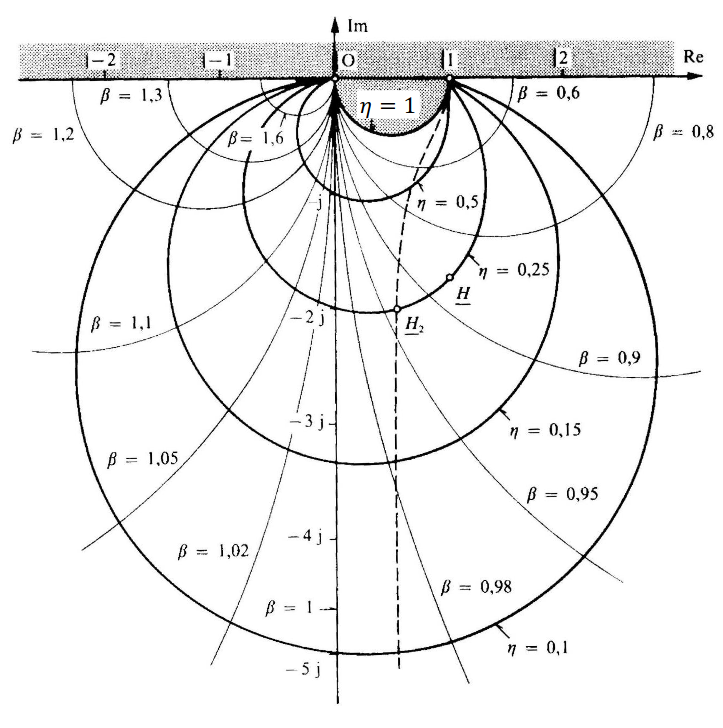
\includegraphics[width=\textwidth]{IMAGES/mecavib/nyquistH.png}
\end{figure}

\subsection{Excitation périodique}
On désire ici résoudre un problème en régime forcé périodique : \begin{equation}
    m \Ddot{x} + c\dot{x} + kx = f(t) = f(t+T)
\end{equation}

Pour cela, on utilise la décomposition de Fourier : \begin{equation}
    f(t) = \frac{F_0}{2} + \sum_{n=0}^\infty (A_n \cos(n\omega t) + B_n \sin(n\omega t)
\end{equation}

Avec pour coefficients : \begin{itemize}
    \item $A_n = \frac{2}{T} \int_0^T f(t) \cos(n\omega t)dt$\\
    \item $B_n = \frac{2}{T} \int_0^T f(t) \sin(n\omega t)dt$\\
\end{itemize}

\warning : \begin{itemize}
    \item si $f$ est paire ($f(t) = f(-t)$) alors $B_n=0$\\
    \item si $f$ est impaire ($f(-t) = -f(t))$ alors $A_n = 0$\\
\end{itemize}

On peut également écrire la forme compacte de l'excitation : \begin{equation}\begin{gathered}
    f(t) = \frac{F_0}{2} + \sum_{n=0}^\infty F_n \cos(n\omega t- \psi_n)\\
    \begin{cases}
        F_n = \sqrt{A_n^2+B_n^2}\\
        \tan \psi_n = \frac{B_n}{A_n}\\
    \end{cases}
    \end{gathered}
\end{equation}

On appelle : \begin{itemize}
    \item \textbf{Fondamentale} : la première harmonique (n=1)\\
    \item \textbf{harmoniques} : n>1\\
\end{itemize}

Par le principe de superposition, on peut sommer les différents déplacements liés aux harmoniques. : \begin{equation}
    x_n = \frac{\frac{F_n}{k}}{\sqrt{(1-(n\beta)^2)^2+4\eta^2(n\beta)^2}} \cos(n \omega t - \psi_n - \varphi_n)
\end{equation}

On a également la décomposition par les complexes : \begin{equation}
    \begin{gathered}
        \underline{f}(t) = \frac{F_0}{2} + \sum_1^\infty F_n e^{-j\psi_n} e^{jn\omega t}\\
        F_n e^{-j\psi_n} = \frac{2}{T} \int_0^T f(t) e^{-jn\omega t}dt\\
        \underline{x}(t) = \frac{F_0}{2k} + \sum_1^\infty \underline{H}(n\omega) \frac{F_n}{k} e^{j(n\omega t-\psi_n)}\\
    \end{gathered}
\end{equation}

\warning Les résultats pour un système en régime permanent sont valables mais il faut remplacer $\beta$ par $n \beta$!\\

Au final, le déplacement réel est donné par : \begin{equation}
    x(t) = \frac{F_0}{2k} + \sum_1^\infty X_n \cos(n\omega t - \psi_n - \varphi_n)
\end{equation}

\subsection{Régime forcé général}
Soit $f$ quelconque : $m\Ddot{x}+c\dot{x}+kx=f(t)$\\
La solution complète est de la forme : $x = x'(t)+x''(t)$ : \begin{itemize}
    \item $x'(t)$ : solution particulière\\
    \item $x''(t)$ : solution générale sans second membre\\
\end{itemize}

\quad \underline{Admittance opérationnelle/fonction de transfert :}\\
\begin{equation}
    Y(s) = \frac{1}{ms^2+cs+k} = \frac{1}{m} \frac{1}{s^2+2\lambda s+\omega_0^2}
\end{equation}

Selon Laplace, la solution générale est : \begin{equation}
\begin{gathered}
    X(s) = Y(s)F(s) + \frac{X_0(s+2\lambda) + V_0}{s^2+2\lambda s+ \omega_0^2}\\
    x(t) = x_a(t) + x_b(t)\\
    \end{gathered}
\end{equation}

\begin{itemize}
    \item $x_a(t)$ : fonction inverse du premier membre ($x_a(t) = \int_0^ty(t-u)f(u)du$) \\
    \item $x_b(t)$ : fonction inverse des termes initiaux\\
\end{itemize}

\subsubsection{Amortissement sur-critique}
($\eta>1$)\\

\begin{equation}
    \begin{gathered}
        Y(s) = \frac{1}{m} \frac{1}{(s-r_1)(s-r_2)}\\
        \text{avec } \begin{cases}
            r_1 = -\lambda + \omega_1\\
            r_2 = -\lambda - \omega_1\\
        \end{cases}
    \end{gathered}
\end{equation}

$x(t) = \frac{1}{m\omega_1} \int_0^t e^{-\lambda u} \sinh{(\omega_1 u)} \cdot f(t-u)du + e^{-\lambda t} (X_0 \cosh{(\omega_1 t)} + \frac{\lambda X_0 + V_0}{\omega_1} \sinh{(\omega_1 t)})$\\

\subsubsection{Amortissement critique}
($\eta=1$)\\

\begin{equation}
    Y(s) = \frac{1}{m} \frac{1}{(s+\omega_0)^2}
\end{equation}
$x(t) = \frac{1}{m}\int_0^t ue^{-\omega_0u} \cdot f(t-u)du + (X_0 + (\omega_0X_0 + V_0)t)e^{-\omega_0t}$\\

\subsubsection{Amortissement sous-critique}
($\eta < 1$)\\

\begin{equation}
    \begin{gathered}
        Y(s) = \frac{1}{m} \frac{1}{s^2 + 2\lambda s+ \omega_0^2} = \frac{1}{m} \frac{1}{(s+\lambda)^2 + \omega_0^2-\lambda^2} = \frac{1}{m\omega_1} \frac{\omega_1}{(s+\lambda)^2+\omega_1^2}\\
        y(t) = \frac{e^{-\lambda t}}{m\omega_1} \sin{\omega_1 t}\\
    \end{gathered}
\end{equation}

$x(t) = \frac{1}{m\omega_1} \int_0^t e^{-\lambda u} \sin{(\omega_1u)}\cdot f(t-u)du + X e^{-\lambda t}\cos{(\omega_1t-\varphi)}$\\
\begin{itemize}
    \item $X = \sqrt{X_0^2 + (\frac{\lambda X_0 + V_0}{\omega_1})^2}$\\
    \item $\tan \varphi = \frac{\lambda X_0 + V_0}{\omega_1 X_0}$\\
\end{itemize}

\subsubsection{Solution de l'impulsion de Dirac}
\begin{equation}
    F\varepsilon = 1 \: (\varepsilon \rightarrow 0, F\rightarrow \infty)
\end{equation}
La transformée de Laplace est donnée par : $F(s) = \mathcal{L}(f(t))=1$\\

La transformée de Laplace de la réponse sous conditions initiales nulles est : $X(s) \equiv D(s) = Y(s)F(s) = Y(s)$\\

\quad \underline{Réponse impulsionnelle en cas d'amortissement sur-critique :}\\
\begin{equation}
    d(t) = \frac{e^{-\lambda t}}{2m\omega_1} (e^{\omega_1 t} - e^{-\omega_1 t}) = \frac{e^{-\lambda t}}{m\omega_1}\sinh(\omega_1 t)
\end{equation}

\quad \underline{Réponse impulsionnelle en cas d'amortissement critique :}\\
\begin{equation}
    d(t) = \frac{t}{m}e^{-\omega_0 t}
\end{equation}

\quad \underline{Réponse impulsionnelle en cas d'amortissement sous-critique :}\\
\begin{equation}
    d(t) = \frac{e^{-\lambda t}}{m\omega_1}\sin(\omega_1 t)
\end{equation}

\subsubsection{Solution de l'échelon de force (step input)}
Définition : $\begin{cases}
    f(t) = 0 & t<0\\
    f(t) = 1 & t>0\\
\end{cases}$, $f(t) = \varepsilon(t)$\\

La transformée de Laplace de la fonction est donnée par : $F(s) = \mathcal{L}(f(t)) = \frac{1}{s}$\\

La transformée de Laplace de la réponse indicielle sous conditions initiales nulles est : $X(s) \equiv E(s) = Y(s) F(s) = \frac{1}{s} Y(s)$\\

\quad \underline{Réponse indicielle en cas d'amortissement sur-critique :}\\
\begin{equation}
    e(t) = \frac{1}{k} (1-e^{-\lambda t}(\cosh{(\omega_1t)} + \frac{\lambda}{\omega_1} \sinh{(\omega_1t)}))
\end{equation}

\quad \underline{Réponse indicielle en cas d'amortissement critique :}\\
\begin{equation}
    e(t) = \frac{1}{k} (1-(1+\omega_0t)e^{-\omega_0t})
\end{equation}

\quad \underline{Réponse indicielle en cas d'amortissement sous-critique :}\\
\begin{equation}
    e(t) = \frac{1}{k} (1-e^{-\lambda t}(\cos(\omega_1t)+\frac{\lambda}{\omega_1} \sin(\omega_1t)))
\end{equation}

On a ainsi la relation : $D(s) = Y(s)1$, $E(s) = Y(s) \frac{1}{s} \Rightarrow D(s) = sE(s) \Rightarrow d(t) = \dot{e}(t)$\\

\subsection{Systèmes avec 2Ddl-libres et conservatifs}
Les coordonnées généralisées d'un système à deux degrés de libertés sont : $x_1(t)$ et $x_2(t)$\\

\begin{equation}
    \begin{gathered}
        m_{11}\Ddot{x}_{1} + c_{11} \dot{x}_{1} + k_{11} x_{1} + m_{12}\Ddot{x}_{2} + c_{12} \dot{x}_{2} + k_{12} x_2 = 0\\
        m_{22}\Ddot{x}_{2} + c_{22} \dot{x}_{2} + k_{22} x_{2} + m_{21}\Ddot{x}_{1} + c_{21} \dot{x}_{1} + k_{21} x_1 = 0\\
        \text{Termes propres }+ \text{ Couplage inertiel } + \text{ Couplage résistif } + \text{ Couplage élastique }\\
    \end{gathered}
\end{equation}

Soit sous forme matricielle : \begin{equation}
    M \Ddot{x} + C \dot{x} + Kx = 0
\end{equation}
Avec : \begin{itemize}
    \item $M$ : la matrice des masses $M = \begin{pmatrix}
        m_{11} & m_{12}\\ m_{21} & m_{22}\\
    \end{pmatrix}$\\
    \item $C$ : la matrice d'amortissement $C = \begin{pmatrix}
        c_{11} & c_{12}\\ c_{21} & c_{22}\\
    \end{pmatrix}$\\
    \item $K$ : la matrice de rigidité $K = \begin{pmatrix}
        k_{11} & k_{12}\\ k_{21} & k_{22}\\
    \end{pmatrix}$\\
\end{itemize}

\subsubsection{Régime libre et conservatif}
On a ici trois ressorts en séries avec deux masses. ($c=0$)\\
\begin{equation}
    M\Ddot{x} + Kx=0
\end{equation}

Les solutions générales du régime libre sont de la forme : \begin{equation}
    \Vec{x} = \Vec{A} e^{pt} \rightarrow \begin{cases}
        x_1 = A_1 e^{pt}\\
        x_2 = A_2 e^{pt}\\
    \end{cases}
\end{equation}

Si ce sont des solutions, alors $Mp^2Ae^{pt} + KAe^{pt} = 0 \Rightarrow \det(Mp^2+K)=0$\\

On pose alors comme solution : \begin{itemize}
    \item $p_I = \pm j \omega_I$\\
    \item $p_{II} = \pm j \omega_{II}$\\
\end{itemize}

On veut alors trouver les $\omega$ tel que : \begin{equation}
    \det(Mp^2+K)=0
\end{equation}

On trouve alors que \begin{itemize}
    \item $A_1 = \begin{pmatrix}
        1\\ \beta_{21}\\
    \end{pmatrix}X_1$\\
    \item $A_2 = \begin{pmatrix}
        1\\ \beta_{22}\\
    \end{pmatrix}X_2$
\end{itemize}

Avec : \begin{equation}
\begin{gathered}
    \beta_{21} = \frac{k_3}{k_2+k_3-m_2\omega_I^2}\\
    \beta_{22} = \frac{k_3}{k_2+k_3-m_2\omega_{II}^2}\\
    \end{gathered}
\end{equation}

Pour trouver les $A_i$ de manière générale, on prend $A_i = \begin{pmatrix}
    1\\ w\\
\end{pmatrix}$ et on trouve $w$ en faisant : \begin{equation}
    (\omega_i^2M-K)A_i = 0
\end{equation}

Une forme des solutions générales du régime libre est : \begin{equation}
    \begin{gathered}
        x_1 = X_1 \cos(\omega_It-\varphi_1) + X_2\cos(\omega_{II}t-\varphi_2)\\
        x_2= \beta_{21}X_1 \cos(\omega_It-\varphi_1) + \beta_{22}X_2\cos(\omega_{II}t-\varphi_2)\\
        \mathbf{x} = \mathbf{\beta}_1X_1\cos(\omega_It-\varphi_1) + \mathbf{\beta}_2X_2\cos(\omega_{II}t-\varphi_2)\\
    \end{gathered}
\end{equation}

Avec les \textbf{vecteurs modaux/vecteurs propres de l'oscillateur} : \begin{itemize}
    \item $\mathbf{\beta}_1 = \begin{pmatrix}
        1\\ \beta_{21}\\
    \end{pmatrix}$\\
    \item $\mathbf{\beta}_2 = \begin{pmatrix}
        1\\ \beta_{22}\\
    \end{pmatrix}$
\end{itemize}

\warning Il y a orthogonalité des modes propres de l'oscillateur : $\beta_1^T M \beta_2 = 0$ et $\beta_1^TK\beta_2 = 0$\\

\centering{\textit{Un mode propre est le mouvement du système lié à une pulsation ou fréquence propre}}
\justifying

\subsubsection{Systèmes symétriques}
Soit $m_1=m_2=m$ et $k_1=k_2=k$\\
On a alors $p^2 = -\frac{k+k_3}{m} \pm \frac{k_3}{m}$ $\Rightarrow \begin{cases}
    \omega_I^2 = \frac{k}{m}\\ \omega_{II}^2 = \frac{k+2k_3}{m}\\
\end{cases}$

Les rapports des amplitudes des solutions valent donc : \begin{itemize}
    \item $\beta_{21} = 1$\\
    \item $\beta_{22} = -1$\\
\end{itemize}

Soit : \begin{itemize}
    \item $x_1 = X_1 \cos(\omega_It-\varphi_1) + X_2 \cos(\omega_{II}t-\varphi_2)$\\
    \item $x_2 = X_1 \cos(\omega_It-\varphi_1) - X_2 \cos(\omega_{II}t-\varphi_2)$\\
\end{itemize}

Le \textbf{premier mode du système} donne donc une oscillation en phase : $x_1 = x_2$\\
Le \textbf{deuxième mode du système} donne des oscillations en opposition de phase : $x_1=-x_2$\\

\subsection{Amortisseur de Frahm}

\begin{figure}[hbt!]
    \centering
    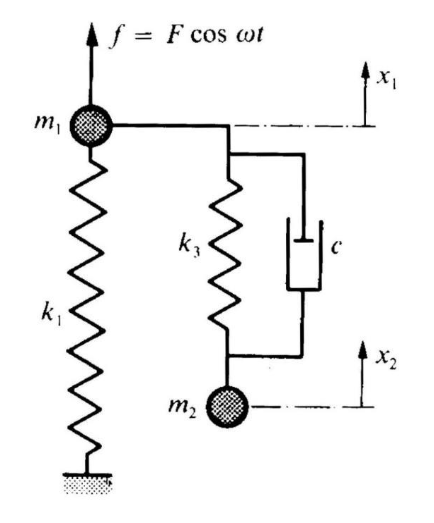
\includegraphics[width=.4\textwidth]{IMAGES/mecavib/frahm.png}
\end{figure}

L'objectif de cet amortisseur est de limiter l'amplitude de $x_1$.\\
On a ici un système à deux degrés de libertés.\\

Les équations du système sont donc : \begin{equation}
    \begin{gathered}
        m_1\Ddot{x}_1 + c(\dot{x}_1-\dot{x}_2) + k_1x_1 + k_3(x_2-x_1) = F\cos{\omega t}\\
        m_2 \Ddot{x}_2 + c(\dot{x}_2-\dot{x}_1)+k_3(x_1-x_2)=0\\
    \end{gathered}
\end{equation}

Les solutions du régime permanent sont données par : \begin{itemize}
    \item $x_1 = X_1 \cos(\omega t-\varphi_1)$ $\Rightarrow \underline{x}_1 = \underline{A}_1 e^{j\omega t}$\\
    \item $x_2 = X_2 \cos(\omega t-\varphi_2)$ $\Rightarrow \underline{x}_2 = \underline{A}_2 e^{j\omega t}$\\
\end{itemize}

Où $\underline{A}_i = X_i e^{-j\varphi_i}$\\

En remplaçant et isolant les variables, on obtient : \begin{equation}
\begin{gathered}
    \underline{A}_1(-\omega^2m_1 + k_1 + k_3 + j\omega c) - \underline{A}_2(k_3 + j\omega c)=F\\
    -\underline{A}_1(k_3+j\omega c) + \underline{A}_2(-\omega^2m_2 + k_3 + j\omega c) = 0\\
    \end{gathered}
\end{equation}

L'amplitude de la grandeur complexe $\underline{A}_1$ relative à l'amplitude du mouvement de la masse principale vaut donc : \begin{equation}
    \begin{gathered}
        \underline{A}_1 = F \frac{(k_3-\omega^2m_2)+j\omega c}{(k_1-\omega^2m_1)(k_3-\omega^2m_2) - \omega^2 m_2k_3 + j\omega c(k_1 - \omega^2(m_1+m_2))}\\
        X_1^2 = \lvert \underline{A}_1\rvert^2\\
    \end{gathered}
\end{equation}

Quelques notations : \begin{itemize}
    \item $\varepsilon = \frac{m_2}{m_1}$, rapport entre la masse de l'amortisseur et la masse principale (dans la pratique << 1)\\
    \item $\omega_1 = \sqrt{\frac{k_1}{m_1}}$ la pulsation propre de l'oscillateur principal\\
    \item $\omega_2 = \sqrt{\frac{k_3}{m_2}}$ la pulsation propre de l'oscillateur secondaire non amorti\\
    \item $\alpha = \frac{\omega_2}{\omega_1}$ rapport entre les pulsations propres, dans la pratique environ 1\\
    \item $\beta = \frac{\omega}{\omega_1}$ rapport entre la pulsation forcée et la pulsation propre de l'oscillateur principal\\
    \item $\eta = \frac{c}{2m_2 \omega_1}$ amortissement relatif croisé\\
    \item $X_{1s} = \frac{F}{k_1}$ déplacement statique de la masse principale\\
    \item $\mu = \frac{X_1}{X_{1s}}$ facteur d'amplification dynamique du mouvement de la masse principale\\
\end{itemize}


\begin{equation}\begin{gathered}
    \mu_1^2 = \frac{4\eta^2\beta^2 + (\beta^2-\alpha^2)^2}{4\eta^2\beta^2(\beta^2(1+\varepsilon)-1)^2+(\varepsilon \alpha^2\beta^2 - (\beta^2-1)(\beta^2-\alpha^2))^2}\\
    \mu_2^2 = \frac{4\eta^2\beta^2 + \alpha^4}{4\eta^2\beta^2(\beta^2(1+\varepsilon)-1)^2+(\varepsilon \alpha^2\beta^2 - (\beta^2-1)(\beta^2-\alpha^2))^2}\\
    \end{gathered}
\end{equation}

On minimise ici $\mu_1$ et non $\mu_2$ qui correspond à l'amplitude relative du mouvement de la masse secondaire.\\

\warning Lorsque $\eta = 0$, les pôles de $\mu^2$ sont les fréquences propres du système.\\

On considère deux cas limites : \begin{itemize}
    \item conservatif (c=0) : $\mu = \frac{\beta^2-\alpha^2}{\varepsilon\alpha^2\beta^2 - (\beta^2-1)(\beta^2-\alpha^2)}$\\
    \item dissipation infinie ($c=\infty$) : $\mu = \frac{1}{\beta^2(1+\varepsilon)-1}$\\
\end{itemize}

\subsubsection{Optimisation}
L'oscillateur de Frahm est optimal s'il y a limitation du mouvement de la masse principale $m_1$ sur une large plage fréquentielle.\\

Il faut choisir une courbe $\mu(\beta)$ passant par deux points P et Q et avec une tangente horizontale en l'un deux.\\

On cherche en premier à déterminer $m_2$ et $k_3$ en posant :\\ 
\begin{equation}
    \begin{gathered}
        \alpha = \frac{1}{1+\varepsilon}\\
        \mu = \sqrt{\frac{2+\varepsilon}{\varepsilon}}
    \end{gathered}
\end{equation}

On détermine ensuite $c$ tel qu'on ait une tangente horizontale de $\mu$ en P ou Q.\\

\subsection{Oscillateur généralisé}
L'équation différentielle matricielle d'un système oscillateur généralisé à n degrés de liberté. \\

\begin{equation}
    [M] \Ddot{x} + [C] \dot{x} + [K] x = f(t)
\end{equation}

Avec : \begin{itemize}
    \item $x$, $\dot{x}$, $\Ddot{x}$ les vecteurs déplacements, vitesses et accélérations\\
    \item $[M]$, $[C]$ et $[K]$, les matrices des masses, d'amortissement et de rigidité\\
    \item $f$ le vecteur des forces extérieures\\
\end{itemize}

\quad \underline{Énergies :}\\

\begin{equation}
    \begin{gathered}
        T = \frac{1}{2}\dot{x}^T[M] \dot{x}\\
        V = \frac{1}{2} x^T[K]x\\
        W = \frac{1}{2}\dot{x}^T[C]\dot{x} \text{ , la fonction de dissipation de Rayleigh}\\
    \end{gathered}
\end{equation}

Soit les équations de Lagrange : \begin{equation}
    \begin{gathered}
        \frac{d}{dt}(\frac{\partial T}{\partial \dot{x}_k}) - \frac{\partial T}{\partial x_k} + \frac{\partial V}{\partial x_k} + \frac{\partial W}{\partial \dot{x}_k} = f_k(t)\\
        \frac{d}{dt}(\frac{\partial T}{\partial \dot{x}}) - \frac{\partial T}{\partial x} + \frac{\partial V}{\partial x} + \frac{\partial W}{\partial \dot{x}} = f(t)\\
    \end{gathered}
\end{equation}

\subsubsection{Conservatif}
Le système peut être simplifié comme : $[M]\Ddot{x} + [K]x=0$\\

En posant : $[A] = [M]^{-1}[K]$ : \textbf{le noyau du système}.\\

\begin{equation}
    \Ddot{x} + [A] x = 0
\end{equation}

Il existe deux moyens de trouver les solutions.\\

\subsubsection{Résolution par solutions particulières}

On pose une solution particulière de la forme : $x = X\cos(\omega t-\varphi)$\\
\begin{equation}
    \Rightarrow ([A]-\delta[I])X = 0
\end{equation}
Avec $\delta = \omega^2$ les pulsations propres du système. Cette équation est valable pour tout X donc : 
\begin{equation}
    det([A]-\delta[I])=0
\end{equation}

On peut également utiliser la forme alternative : \begin{equation}
    \begin{gathered}
        \alpha M \Ddot{x} + Ix = 0\\
        det(\alpha M - \tau I)=0\\
        \tau = \frac{1}{\omega^2}\\
    \end{gathered}
\end{equation}

On ordonne ensuite les solutions de l'équation caractéristique et des pulsations propres : \begin{equation}
    \omega_I<\dots <\omega_N
\end{equation}

Ainsi, $\Vec{x}_p = \Vec{X}_p \cos(\omega_pt-\varphi_p)$\\

On pose $\Vec{X}_p = \Vec{\beta}_pX_p$ avec $X_p$ une amplitude de référence déterminée par les conditions initiales.\\

\warning On pose toujours le premier élément de $\Vec{\beta}$ comme 1\\

La solution générale est donc une combinaison linéaire de tous les modes : $\Vec{x}(t) = \sum_{p=1}^n \Vec{\beta}_pX_p \cos(\omega_pt-\varphi_p)$\\

\subsubsection{Résolution dans la base modale}

La résolution intervient ici par changement de base dans la base modale.\\

La matrice de changement de base est donnée par : $x = [B]q$ avec : \begin{itemize}
    \item $q_p$ : les coordonnées normales ou modales de rang p\\
    \item $[B] = (\Vec{\beta}_1, \dots, \Vec{\beta}_n)$ \\
\end{itemize}

Dès lors : \begin{equation}
    \begin{gathered}
        \left[M \right] \left[B\right]\Ddot{q} + [K][B]q = 0\\
        \Rightarrow [B]^T[M][B]\Ddot{q} + [B]^T[K][B]q = 0\\
        \Rightarrow [M^0] \Ddot{q} + [K^0]q = 0\\
    \end{gathered}
\end{equation}

Les matrices $[M^0]$ et $[K^0]$ sont diagonales et symétriques. On a donc \textbf{un découplage des n équations}.\\
Il y a cependant des conditions nécessaire et suffisante pour l'existence de B : M et K symétriques et M et/ou K définies strictement positives.\\

Ainsi, on obtient n équations découplées : $\Ddot{q}_p + \delta_p q_p = 0$ avec $\omega_p^2 = \delta_p = \frac{k_p^0}{m_p^0}$\\

L'expression matricielle devient alors : \begin{equation}\begin{gathered}
    \Ddot{q} + [B]^{-1}[M]^{-1}[K][B]q = 0\\
    \Ddot{q} + [\Delta] q = 0
    \end{gathered}
\end{equation}

Avec $[\Delta]$ la matrice des valeurs propres de A, soit les pulsations propres au carré.\\

Ainsi : $[\Delta] = [B]^{-1}[A][B] = [M^0]^{-1}[K^0]$\\

L'intégration nous donne : $q_p = Q_p \cos(\omega_pt-\varphi_p)$\\

\begin{equation}
    x(t) = [B]q = \sum_{p=1}^n \Vec{\beta}_p Q_p \cos(\omega_pt-\varphi_p)
\end{equation}

\quad \underline{Energies dans la base modale :}\\
\begin{equation}
    \begin{gathered}
        T = \frac{1}{2}\dot{q} [M^0]\dot{q} = \frac{1}{2}\sum_p^n m_p^0\dot{q}_p^2\\
        V = \frac{1}{2}q^T[K^0]q = \frac{1}{2} \sum_p^n k_p^0 q_p^2\\
    \end{gathered}
\end{equation}

\quad \underline{Orthogonalité des vecteurs modaux :}\\

\begin{equation}
    \begin{gathered}
        \beta_r^T [M] \beta_s = \delta_{rs} m_r^0\\
        \beta_r^T [K] \beta_s = \delta_{rs} k_r^0\\
    \end{gathered}
\end{equation}

\quad \underline{Normalisation des vecteurs modaux :}\\
Plusieurs possibilités : \begin{itemize}
    \item Valeur unité attribuée à l'amplitude de la première variable du vecteur\\
    \item Valeur unité attribuée à la plus grande des amplitudes\\
    \item Norme unitaire du vecteur $\lvert \lvert \beta_p\rvert \rvert = 1$\\
\end{itemize}

\quad \underline{Réponse aux conditions initiales :}\\
\begin{itemize}
    \item $x(0) = X_0 = \sum_p^n \beta_p X_p \cos\varphi_p$\\
    \item $\dot{x}(0)= V_0 = \sum_p^n \beta_p\omega_p X_p \sin\varphi_p$\\
\end{itemize}

En multipliant le tout par $\beta_r^T [M]$, on a : \begin{itemize}
    \item $X_r \cos\varphi_r = \frac{1}{m_r^0} \beta_r^T [M] X_0$\\
    \item $X_r \sin\varphi_r = \frac{1}{m_r^0 \omega_r} \beta_r^T [M] V_0$\\
\end{itemize}

\begin{equation}
    x = \sum_p^n \frac{1}{m_p^0} \beta_p (\beta_p^T[M]X_0 \cos(\omega_pt) + \frac{1}{\omega_p} \beta_p^T [M] V_0 \sin(\omega_pt))
\end{equation}

Cas particuliers : \begin{itemize}
    \item Déplacement initial proportionnel à un vecteur modal et vitesse nulle ($X_0 = X\beta_r$, $V_0 = 0$) : $x = X\beta_r \cos(\omega_rt)$\\
    \item Vitesse et déplacement initial proportionnel à un vecteur modal : $x = \sqrt{X^2 + (\frac{V}{\omega_r})^2} \beta_r \cos(\omega_rt-\varphi_r)$ et $\tan\varphi_r = \frac{V}{X\omega_r}$\\
\end{itemize}

\quad \underline{Quotient de Rayleigh :}\\
Pour un vecteur $u$ quelconque : \begin{equation}
    R(u) = \frac{u^T[K] u}{u^T[M]u}
\end{equation}

Pour un vecteur modal : $R(\beta_p) = \omega_p^2$\\

Pour un vecteur $u$ qui s'écrit comme combinaison linéaire des vecteurs modaux $\beta_p$ : $R(u) = R([B]\gamma) = \frac{\gamma^T[\Delta]\gamma}{\gamma^T\gamma}$\\
Sous la condition : $[B]^T[M][B] = [I]$, $[B]^T[K][B] = [\Delta]$\\

Valeur du quotient de Rayleigh au voisinage d'un vecteur modal : $R(u) = \frac{\delta_r + \sum_{p\neq r}^n \delta_p \varepsilon_p^2}{1+\sum_{p\neq r}^n \varepsilon_p^2} \simeq \delta_r + \sum_{p\neq r}^n (\delta_p-\delta_r)\varepsilon_p^2$\\

\quad \underline{Théorème d'encadrement :} $\delta_1 \leq R(u) \leq \delta_n$

\subsubsection{Dissipatif et libre}
L'équation différentielle de l'oscillateur généralisé à n degrés de liberté en régime libre dissipatif vaut : \begin{equation}
    [M]\Ddot{x} + [C] \dot{x} + [K]x = 0
\end{equation}
Avec : $[C]$ la matrice des pertes.\\

De nouveaux, on à la résolution du régime libre dissipatif par changement de base : $x = [B]q$\\

Soit : \begin{equation}
\begin{gathered}
    \left[B\right]^T[M][B]\Ddot{q} + [B]^T[C][B]\dot{q} + [B]^T[K][B]q = 0\\
    [M^0] \Ddot{q} + [C^0]\dot{q} + [K^0]q = 0\\
    \end{gathered}
\end{equation}

\warning Les matrices $[M^0]$, $[C^0]$, $[K^0]$ sont diagonales si elles respectent les conditions de Caughey.\\

\quad \underline{Condition de Caughey :}\\

\begin{itemize}
    \item Condition nécessaire et suffisante d'existence d'une matrice $[B]$ diagonalisant simultanément $[M]$, $[C]$ et $[K]$ : $[C][M]^{-1}[K] = [K][M]^{-1}[C]$\\
    \item Condition suffisante mais non nécessaire : $[M]^{-1}[C] = \sum_{i=0}^{n-1} \alpha_i [[M]^{-1}[K]]^i$
\end{itemize}

\footnote{Cas particulier de l'amortissement ou frottement proportionnel : $[C] = \alpha [M] + \alpha_1 [K]$}

Conséquences d'un amortissement satisfaisant la condition de Caughey : \begin{itemize}
    \item résolution du régime libre dissipatif selon la démarche modale des systèmes conservatifs\\
    \item matrice $[B]$ identique\\
    \item n modes vibratoires amortis réels dit "classiques"\\
\end{itemize}

\quad \underline{Solution en base modale :}\\
\begin{equation}
\begin{gathered}
    \Ddot{q} + [2\Lambda] \dot{q} + [\Omega_0^2] q = 0\\
    [2\Lambda] = [B]^{-1}[M]^{-1}[C][B]\\
    [\Omega_0^2] = [B]^{-1}[M]^{-1} [K][B]\\
    \end{gathered}
\end{equation}

Comme les matrices sont diagonales, on a un découplage du système différentiel en n équations indépendantes : $\Ddot{q}_p + 2\lambda_p \dot{q}_p + \omega_{0p}^2q_p = 0$\\
Avec : $2\lambda_p = \frac{c_p^0}{m_p^0}$ et $\omega_{0p}^2 = \delta_p = \frac{k_p^0}{m_p^0}$\\

La solutions des n équations découplées est donc : \begin{equation}
    q_p = Q_p e^{-\lambda_p t}\cos(\omega_p t-\varphi_p)
\end{equation}

La \textbf{pulsation propre $\omega_p$ de rang p du système amorti} : \begin{equation}
    \omega_p = \omega_{0p} \sqrt{1-\eta_p^2}
\end{equation}

Avec : \begin{itemize}
    \item $\lambda_p$ coefficient d'amortissement modal\\
    \item $\eta_p = \frac{\lambda_p}{\omega_{0p}}$ l'amortissement relatif/facteur d'amortissement modal\\
\end{itemize}

Soit la solution globale : $x = \sum_p^n \beta_p X_p e^{\lambda_p t} \cos(\omega_p t-\varphi_p)$\\

Conditions d'un lâcher initial : $X_0 = \sum_p^n \beta_p X_p \cos\varphi_p$ et $V_0 = \sum_p^n \beta_p X_p (\omega_p \sin \varphi_p - \lambda_p \cos\varphi_p)$\\

Solution générale : \begin{equation}
    x(t) = \sum_{p=I}^n \frac{1}{m_p^0} \beta_p e^{-\lambda_p t} (\beta_p^T [M]X_0 \cos(\omega_p t) + \frac{1}{\omega_p} \beta_p^T [M](V_0 + \lambda_p X_0)\sin(\omega_p t))
\end{equation}

\quad \underline{Système ne satisfaisant pas Caughey :}\\
On recherche alors une solution approchée. On utilise le concept du quotient de Rayleigh : \\
\begin{equation}
    R_\lambda(\beta_p) = \frac{1}{2} \frac{\beta_p^T [C]\beta_p}{\beta_p^T [M]\beta_p} = \lambda_p = \frac{c_p^0}{2 m_p^0}
\end{equation}
$k_p^0 = \beta_p^T [K] \beta_p$\\

Grâce à cela, on peut trouver les $c_p^0$, $m_p^0$ et $k_p^0$.\\
\warning On suppose d'abord ici le système conservatif; on trouve les pulsations propres du système ainsi que les vecteurs propres qui sont approximativement les mêmes dans les deux systèmes. Puis on trouve les autres valeurs.\\

\subsubsection{Conservatif Forcé}

On a l'équation matricielle : \begin{equation}
    [M]\Ddot{x}(t) + [K] x(t) = f(t)
\end{equation}

Où $f(t)$ est le vecteur d'ordre n des forces externes. Dans la base modale, on a : \begin{equation}
    [M^0] \Ddot{q} + [K^0] q = [B]^T f = f^0
\end{equation}
Avec $f^0$ le vecteur des forces modales.\\

Dès lors : \begin{equation}
    \Ddot{q} + [\Delta] q = [M^0]^{-1} f^0
\end{equation}
Avec $[\Delta] = [\Omega^2]$ la matrice diagonale des carrés des pulsations propres.\\
On a alors un \textbf{découplage} du régime forcé en n équations indépendantes. La résolution des n équations par la méthode de Laplace est (condition initiale nulle): \begin{equation}
    q_p = \frac{1}{m^0_p \omega_{0p}} \int_0^t f_p^0 (t-u) \sin\omega_{0p}udu
\end{equation}

Soit la solution générale du régime forcé avec conditions initiales : \begin{equation}
    x = \sum_p^n \frac{1}{m_p^0} \beta_q (\frac{1}{\omega_{0p}} \int_0^t f_p^0(t-u)\sin \omega_{0p} u du + \beta_p^T [M] X_0 \cos \omega_{0p} t + \frac{1}{\omega_{0p}} \beta_p^T [M] V_0 \sin\omega_{0p}t)
\end{equation}

\subsubsection{Dissipatif forcé}
Dans la base modale : \begin{equation}
    \Ddot{q} + [2\Lambda] \dot{q} + [\Delta] q = [M^0]^{-1} F^0(t)
\end{equation}
Avec $F^0 = [B]^T F$\\

On a dès lors de nouveau un découplage de n équations.\\
Équation du mode de rang p : $\Ddot{q}_p + 2 \lambda_p \dot{q}_p + \omega_{0p}^2 q_p = \frac{1}{m_p^0} f_p^0(t)$\\
Avec : \begin{itemize}
    \item $\lambda_p = \frac{c_p^0}{2m_p^0}$\\
    \item $\eta_p = \frac{\lambda_p}{\omega_{0p}}$\\
    \item $\omega_p = \omega_{0p} \sqrt{1-\eta_p^2}$\\
\end{itemize}

La solution dans la base modale est donnée par : \begin{equation}
    q_p(t) = \frac{1}{m_p^0 \omega_p} \int_0^t f_p^0 (t-u)\sin(\omega_p u)du + \frac{e^{-\lambda_p t}}{m_p^0} (\beta_p^T [M] X_0 \cos(\omega_p t) + \frac{1}{\omega_p} \beta_p^T [M] (V_0+\lambda_p X_0)\sin(\omega_p t))
\end{equation}

Si la force externe est permanente (harmonique), alors on peut utiliser le domaine de Fourier et définir une fonction de transfert.\\
\begin{equation}
    \begin{gathered}
        Q_p(j\omega) = Y_{pp}^0(j\omega) F_p^0(j\omega)\\
        Y_{pp}^0 (j\omega) = \frac{1}{m_p^0(\omega_{0p}^2 + 2j\eta_p \omega_{op}\omega - \omega^2)}\\
    \end{gathered}
\end{equation}

On peut alors retourner en base physique : \begin{equation}
    X(j\omega) = [Y](j\omega) F(j\omega) =[ \sum_{p=I}^n \frac{\beta_p \beta^T_p}{m_p^0(\omega_{0p}^2 + 2j\eta_p \omega_{op}\omega - \omega^2)}]F(j\omega)
\end{equation}
Où $[Y](j\omega)$ est la fonction de réponse en fréquence (FRF).\\
On définit alors $Y_{rs}$ comme le déplacement du point r due à la force au point s.\\
\begin{equation}
    Y_{rs} = \sum_{p=I}^n \frac{\beta_r^p \beta_s^p}{m_p^0(\omega_{0p}^2 + 2j\eta_p \omega_{op}\omega - \omega^2)}
\end{equation}
Au voisinage du point p, on a : $Y_{rs} = Y_{rs}^I + \dots + Y_{rs}^n \simeq Y_{rs}^p$\\

\subsubsection{Matrice de Compliance}
Lorsque l'on étudie des poutres, on utilise de préférence la matrice de compliance : \begin{equation}
    [\alpha] = \begin{pmatrix}
        \delta_1 & \delta_{21} & \dots\\
        \delta_{21} & \delta_2 \dots\\
        \vdots & \vdots & \delta_n\\
    \end{pmatrix}
\end{equation}
Qui est symmétrique! Chaque delta est calculé en mettant une force externe P=1 sur une des masses du système et en calculant son influence sur toutes les masses.\\

Suite à cela, on peut calculer l'inverse des fréquences propres du système comme : \begin{equation}
    ([\alpha] [M] - I\tau) \beta = 0
\end{equation}
On peut donc réécrire $[K] = [\alpha]^{-1}$\\

\subsection{Systèmes continus}
\subsubsection{2nd ordre}
Les masses sont réparties et déformables. Les éléments dissipatifs et élastiques sont continus. Les systèmes possèdent un nombre infini de degrés de libertés.\\

\textbf{Équation d'onde de d'Alembert} : \begin{equation}
    \frac{\partial^2y}{\partial t^2} = a^2 \frac{\partial^2y}{\partial x^2}
\end{equation}
Avec : \begin{itemize}
    \item $y(x,t)$ la fonction vibratoire\\
    \item $x$ la variable géométrique (m)\\
    \item $t$ temps (s)\\
    \item $a$ la célérité de l'onde dans le milieu (m/s)\\
\end{itemize}

\quad \underline{Vibrations latérales d'une corde :}\\
Soit $\mu_1$ la masse de la corde par unité de longueur, constante et concentrée sur la ligne moyenne. \\
On a ici l'équation : \begin{equation}
    \frac{\partial^2y}{\partial t^2} = \frac{T}{\mu_1} \frac{\partial^2y}{\partial x^2}
\end{equation}

\quad  \underline{Vibrations longitudinales d'une barre :}\\
Soit $\varepsilon = \frac{\partial u}{\partial x}$ l'élongation de la barre.\\

\begin{equation}
    \frac{\partial^2u}{\partial t^2} = \frac{E}{\rho} \frac{\partial^2u}{\partial x^2}
\end{equation}

\quad \underline{Résolution par séparation de variables :}\\

Soit $y(x,t) = V(x)U(t)$\\
\begin{equation}\begin{gathered}
    \frac{\Ddot{U}}{U} = a^2 \frac{\Ddot{V}}{V} = -\omega_n^2\\
    U_n(t) = A_n \cos(\omega_n t) + B_n \sin(\omega_n t)\\
    V_n(x) = C_n \cos(\alpha_n x) + D_n \sin(\alpha_n x)\\
    \alpha_n = \frac{\omega_n}{a}\\
    \end{gathered}
\end{equation}

La solution générale est donc donnée par : \begin{equation}
    y(x,t) = \sum_{n=1}^\infty (C_n \cos(\alpha_n x) + D_n \sin(\alpha_n x))(A_n \cos(\omega_n t) + B_n \sin(\omega_n t))
\end{equation}
Chacun des modes du système doivent répondre aux conditions de bord.\\
Les conditions aux limites doivent être homogènes. La partie non homogène des conditions aux limites est satisfaite par une déformée statique que l'on superpose à la solution vibratoire.

\warning Les termes en x dans la solution générales font référence aux $\beta$ des systèmes généralisés. Comme nous l'avons fait auparavant, on met également les amplitudes du membre spatial égales à 1 afin de normaliser la solution.\\

\subsubsection{4ème ordre}
On utilise la théorie de \textbf{Bernoulli-Euler} des poutres droites afin d'étudier les vibrations de flexion de celles-ci.\\
L'axe neutre x de la poutre est une droite; elle vibre latéralement dans le plan xy; les axes y et z sont principaux d'inertie; l'inertie de rotation des sections droites de la poutre est négligée et enfin, une section droite avant déformation reste droite après déformation.\\

Ici, l'équation des ondes est donnée par : \begin{equation}
    \begin{gathered}
        \mu_1 \frac{\partial^2y}{\partial t^2} = -\frac{\partial^2 M_f}{\partial x^2}\\
        \frac{\partial^2y}{\partial x^2} = \frac{M_f}{EI}\\
        \frac{\partial^2y}{\partial t^2} = - \frac{EI}{\mu_1} \frac{\partial^4 y}{\partial x^4}\\
    \end{gathered}
\end{equation}

\quad \underline{Séparation de variables :}\\
De nouveau, $y(x,t) = V(x)U(t)$\\
\begin{equation} \begin{gathered}
    \frac{\Ddot{U}}{U} = -\frac{EI}{\mu_1} \frac{V^{(4)}}{V}\\
    U_n(t) = A_n \cos(\omega_n t) + B_n \sin(\omega_n t)\\
    V_n(x) = C_{n1} e^{\alpha_nx} + C_{n2} e^{-\alpha_n x} + C_{n3} \cos(\alpha_n x) + C_{n4} \sin(\alpha_n x) \\= D_{n1} \cosh(\alpha_nx) + D_{n2} \sinh(\alpha_n x) + C_{n3} \cos(\alpha_n x) + C_{n4} \sin(\alpha_n x)\\
    \alpha_n = \sqrt[4]{\omega_n^2 \frac{\mu_1}{EI}}\\
    \end{gathered}
\end{equation}

La solution générale est donc : \begin{equation}
        y(x,t) = \sum_{n=1}^\infty U_n(t) V_n(x)
\end{equation}
\footnote{Lors d'une torsion, on a : $\frac{\partial^2 \varphi}{\partial t^2} = \frac{G I_p}{I_p \rho} \frac{\partial^2 \varphi}{\partial x^2}$, on a par ailleurs $dJ = \rho dx I_p$}
On étudie quatre types d'appuis (conditions de bord) : \begin{table}[hbt!]
    \centering
    \begin{tabular}{c|c|c|c|c|c|c}
        Appuis & $M_f$ & $Q$ & $y$ & $\dot{y}$ & $\Ddot{y}$ & $y^{(3)}$ \\
        \hline
        Appuis simple & $0$ & & 0 & & 0 & \\
        \hline
        Encastrement parfait & & & 0 & 0& \\ \hline
        Extrémité libre & 0 & 0 & & & 0& 0\\ \hline
        Encastrement partiel élastique & $-k\dot{y}$ & & 0 & & $\frac{k}{EI} \dot{y}$ & \\
    \end{tabular}
\end{table}




\end{document}